%%%%%%%%%%%%%%%%%%%%%%%%%%%%%%%%%%%%%%%%%%%%%%%%%%%%%%%%%%%%%%%%%%%%%%%%%%%

\documentclass{standalone}

\usepackage{amsmath}
\usepackage{mathptmx}
\usepackage{tikz}
\usetikzlibrary{external}
\tikzexternalize{complete-square-a1-c0}

%% IEEE uses Times Roman font, so we'll default to Times.
%% These three commands make up the entire times.sty package.
\renewcommand{\rmdefault}{ptm}
\renewcommand{\ttdefault}{pcr}
\normalfont\selectfont

%%%%%%%%%%%%%%%%%%%%%%%%%%%%%%%%%%%%%%%%%%%%%%%%%%%%%%%%%%%%%%%%%%%%%%%%%%%
%% Completing the square for the function f(x) = x^2 + bx.
%%%%%%%%%%%%%%%%%%%%%%%%%%%%%%%%%%%%%%%%%%%%%%%%%%%%%%%%%%%%%%%%%%%%%%%%%%%

\begin{document}

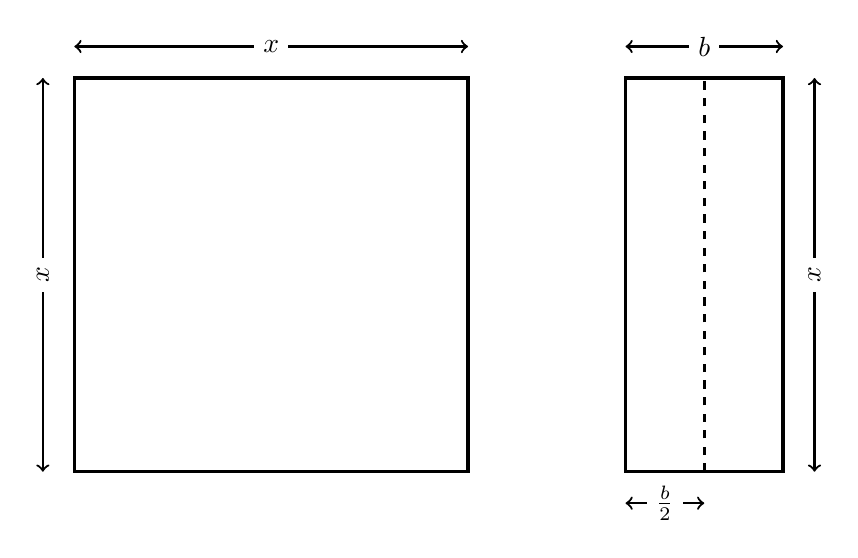
\begin{tikzpicture}[%%
  arrowStyle/.style={<->,thick},%%
  dashStyle/.style={-,dashed,very thick},%%
  labelStyle/.style={fill=white},%%
  lineStyle/.style={-,very thick}%%
]
%%
%%
\pgfmathsetmacro{\bside}{2}
\pgfmathsetmacro{\dbx}{2}  %% the gap between x^2 and bx
\pgfmathsetmacro{\dx}{0.4}
\pgfmathsetmacro{\dy}{\dx}
\pgfmathsetmacro{\xlow}{0}
\pgfmathsetmacro{\xside}{5}
\pgfmathsetmacro{\ylow}{\xlow}
%% For the rectangle bx.
\pgfmathsetmacro{\bend}{\xside+\dbx+\bside}
\pgfmathsetmacro{\bstart}{\xside+\dbx}
%%
%% Coordinates for the square x^2.
\coordinate (xlowerLeft) at (\xlow,\ylow);
\coordinate (xupperRight) at (\xside,\xside);
%% Coordinate for the rectangle bx.
\coordinate (blowerLeft) at (\xside+\dbx,\ylow);
\coordinate (bupperRight) at (\xside+\dbx+\bside,\xside);
%%
\normalsize
%% Draw and label the square for x^2.
%% Draw the square for x^2.
\draw[lineStyle] (xlowerLeft) rectangle (xupperRight);
%% Label the length of the square x^2.
\draw[arrowStyle] (\xlow,\xside+\dx) -- (\xside,\xside+\dx);
\node[labelStyle] at (\xside/2,\xside+\dx) {$x$};
%% Label the width of the square x^2.
\draw[arrowStyle] (\xlow-\dx,\ylow) -- (\xlow-\dx,\xside);
\node[labelStyle,rotate=90] at (\xlow-\dx,\xside/2) {$x$};
%%
%% Draw and label the rectangle bx.
%% Draw the rectangle for bx.
\draw[lineStyle] (blowerLeft) rectangle (bupperRight);
%% Label the length of the rectangle bx.
\draw[arrowStyle] (\bstart,\xside+\dy) -- (\bend,\xside+\dy);
\node[labelStyle] at (\xside+\dbx+\bside/2,\xside+\dy) {$b$};
%% Label the width of the rectangle bx.
\draw[arrowStyle] (\bend+\dx,\ylow) -- (\bend+\dx,\xside);
\node[labelStyle,rotate=90] at (\bend+\dx,\xside/2) {$x$};
%%
%% Half the rectangle bx.
\draw[dashStyle] (\bstart+\bside/2,\ylow) -- (\bstart+\bside/2,\xside);
%% Label the half width of the rectangle.
\draw[arrowStyle] (\bstart,-\dy) -- (\bstart+\bside/2,-\dy);
\node[labelStyle] at (\bstart+\bside/4,-\dy) {$\frac{b}{2}$};
\end{tikzpicture}

\end{document}
